\documentclass[tikz,border=2mm]{standalone}
\usetikzlibrary{arrows.meta}

\begin{document}

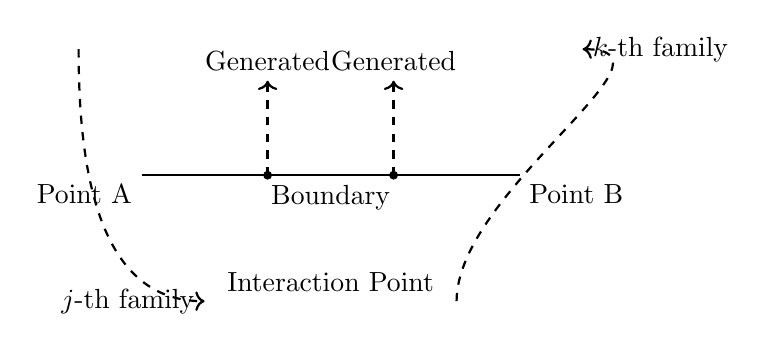
\begin{tikzpicture}[scale=0.8]
    % Define coordinates for the boundaries
    \coordinate (B1) at (0,0);
    \coordinate (B2) at (6,0);

    % Draw the boundary
    \draw[thick] (B1) -- node[midway, below] {Boundary} (B2);

    % Draw the j-th family wave front (left)
    \draw[dashed, thick, ->] (-1,2) to[out=-90,in=180] (1,-2) node[left] {$j$-th family};

    % Draw the k-th family wave front (right)
    \draw[dashed, thick, ->] (5,-2) to[out=90,in=0] (7,2) node[right] {$k$-th family};

    % Draw the interaction points and generated wave fronts
    \foreach \x/\y in {2/0, 4/0} {
        \fill (\x,\y) circle (2pt);
        \draw[dashed, thick, ->] (\x,\y) -- ++(0,1.5) node[above] {Generated};
    }

    % Add labels and annotations
    \node[below left] at (0,0) {Point A};
    \node[below right] at (6,0) {Point B};
    \node[above] at (3,-2) {Interaction Point};
\end{tikzpicture}

\end{document}